\documentclass[tikz]{standalone}
\usepackage{pgfplots}
\pgfplotsset{compat=1.15}
\usepackage{mathrsfs}
\usetikzlibrary{arrows,calc}
\usepackage{tkz-euclide}
\pagestyle{empty}

\definecolor{AngleClr}{rgb}{0,0.39215686274509803,0}
\definecolor{ShapeClr}{rgb}{0.6,0.2,0}

\begin{document}

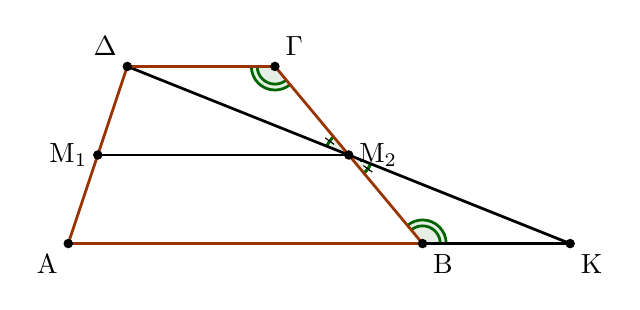
\begin{tikzpicture}[scale=.75]
\tkzSetUpLine[line width=1pt,color=black]
\tkzSetUpPoint[fill=black]

\tkzDefPoints{0/0/A,6/0/B,1/3/D,3.5/3/C}

\tkzDefMidPoint(A,D) \tkzGetPoint{M1}
\tkzDefMidPoint(B,C) \tkzGetPoint{M2}

\tkzDefPointBy[symmetry=center M2](D)\tkzGetPoint{K}

\tkzFillPolygon[fill=white](A,B,C,D)

\tkzFillAngles[fill=AngleClr,size=.4,fill opacity=0.1](C,M2,D B,M2,K)
\tkzMarkAngles[line width=1pt,color=AngleClr,size=.4](C,M2,D B,M2,K)
\tkzMarkAngles[mark=|,mksize=2,line width=1pt,size=.4,color=AngleClr](C,M2,D B,M2,K)

\tkzFillAngles[fill=AngleClr,size=.4,fill opacity=0.1](D,C,M2 K,B,M2)
\tkzMarkAngles[line width=1pt,color=AngleClr,size=.3](D,C,M2 K,B,M2)
\tkzMarkAngles[line width=1pt,color=AngleClr,size=.4](D,C,M2 K,B,M2)

\tkzDrawSegments(M1,M2 D,K B,K)

\tkzDrawPolygon[color=ShapeClr](A,B,C,D)
\tkzDrawPoints[size=3](A,B,C,D,K,M1,M2)
\tkzLabelPoint[below left](A){$\rm A$}
\tkzLabelPoint[below right](B){$\rm B$}
\tkzLabelPoint[above right](C){$\rm \Gamma$}
\tkzLabelPoint[above left](D){$\rm \Delta$}
\tkzLabelPoint[below right](K){$\rm K$}
\tkzLabelPoint[left](M1){$\rm M_1$}
\tkzLabelPoint[right](M2){$\rm M_2$}

\end{tikzpicture}
\end{document}
